\section{Objeto de estudio}

El objeto no es un banco ni BIAN entero. Son los contratos OpenAPI con los que el sector describe sus APIs. Quedan fuera del objeto la organización BIAN, el código de los backends y la infraestructura. BIAN entra como modelo de referencia.

\begin{figure}[H]
  \centering
  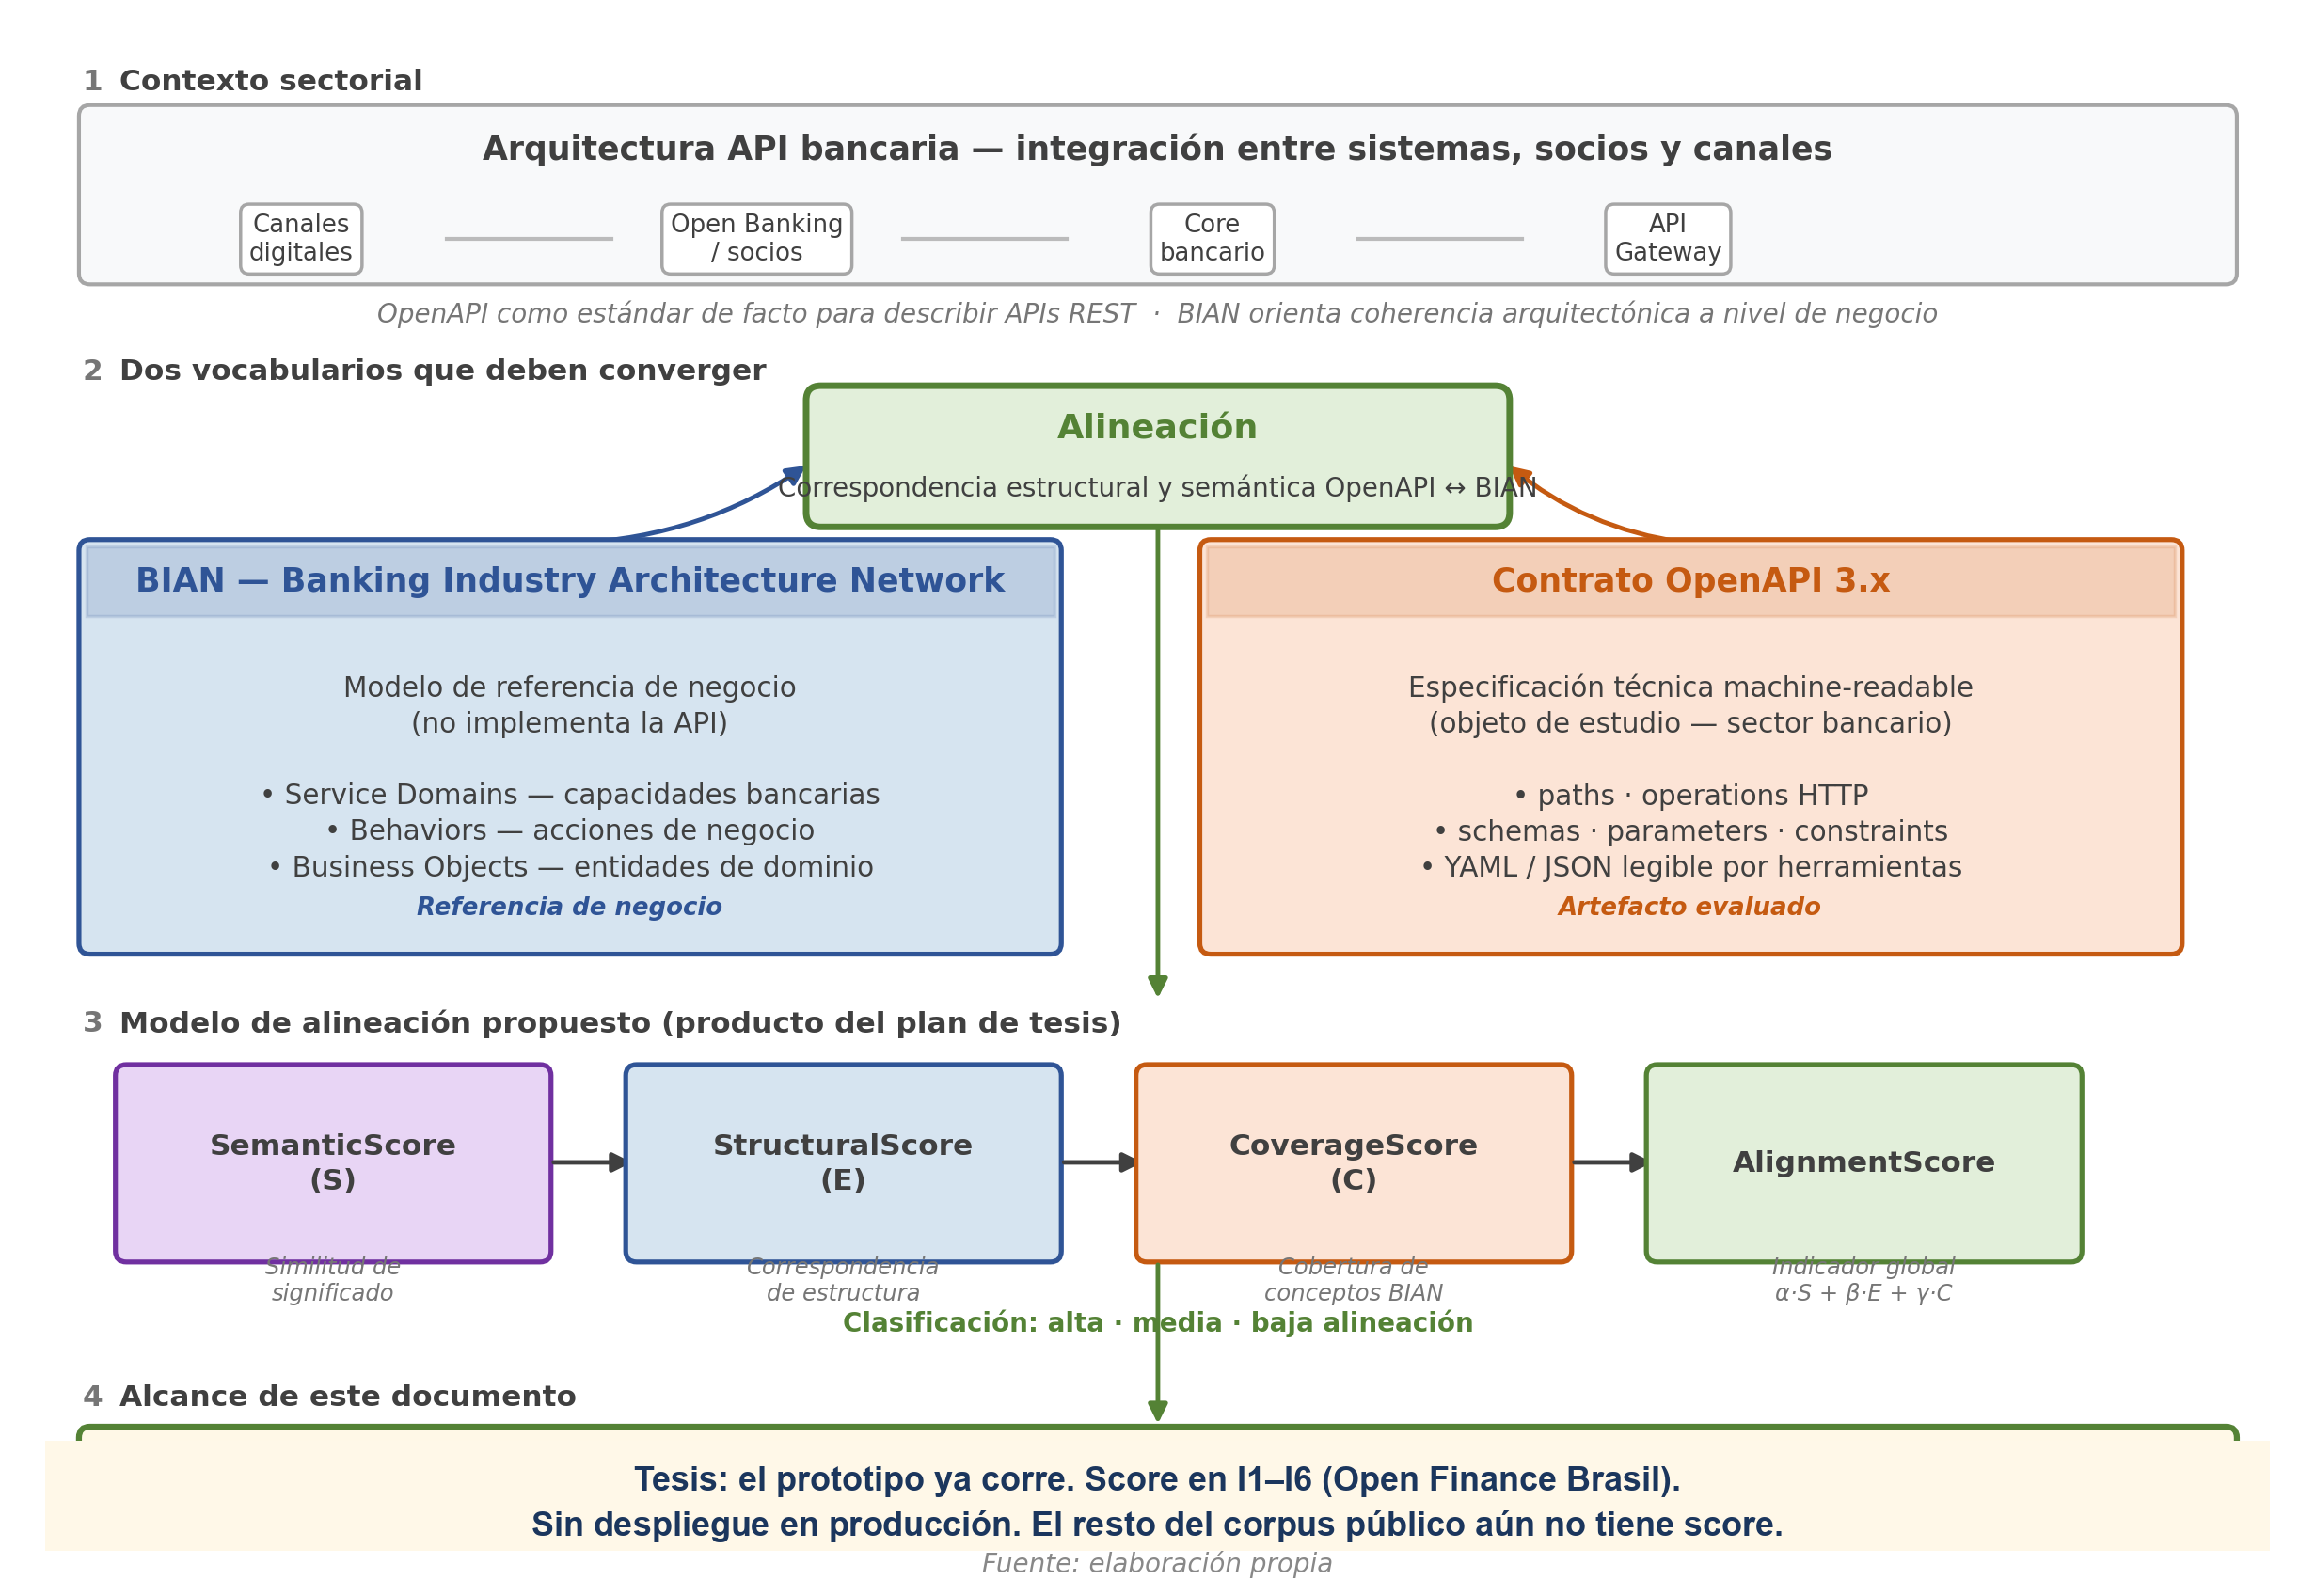
\includegraphics[width=0.92\textwidth]{Figura_01_Contexto}
  \caption{Contexto: arquitectura API bancaria, BIAN, OpenAPI y modelo S/E/C}
  \label{fig:contexto}
\end{figure}

\begin{figure}[H]
  \centering
  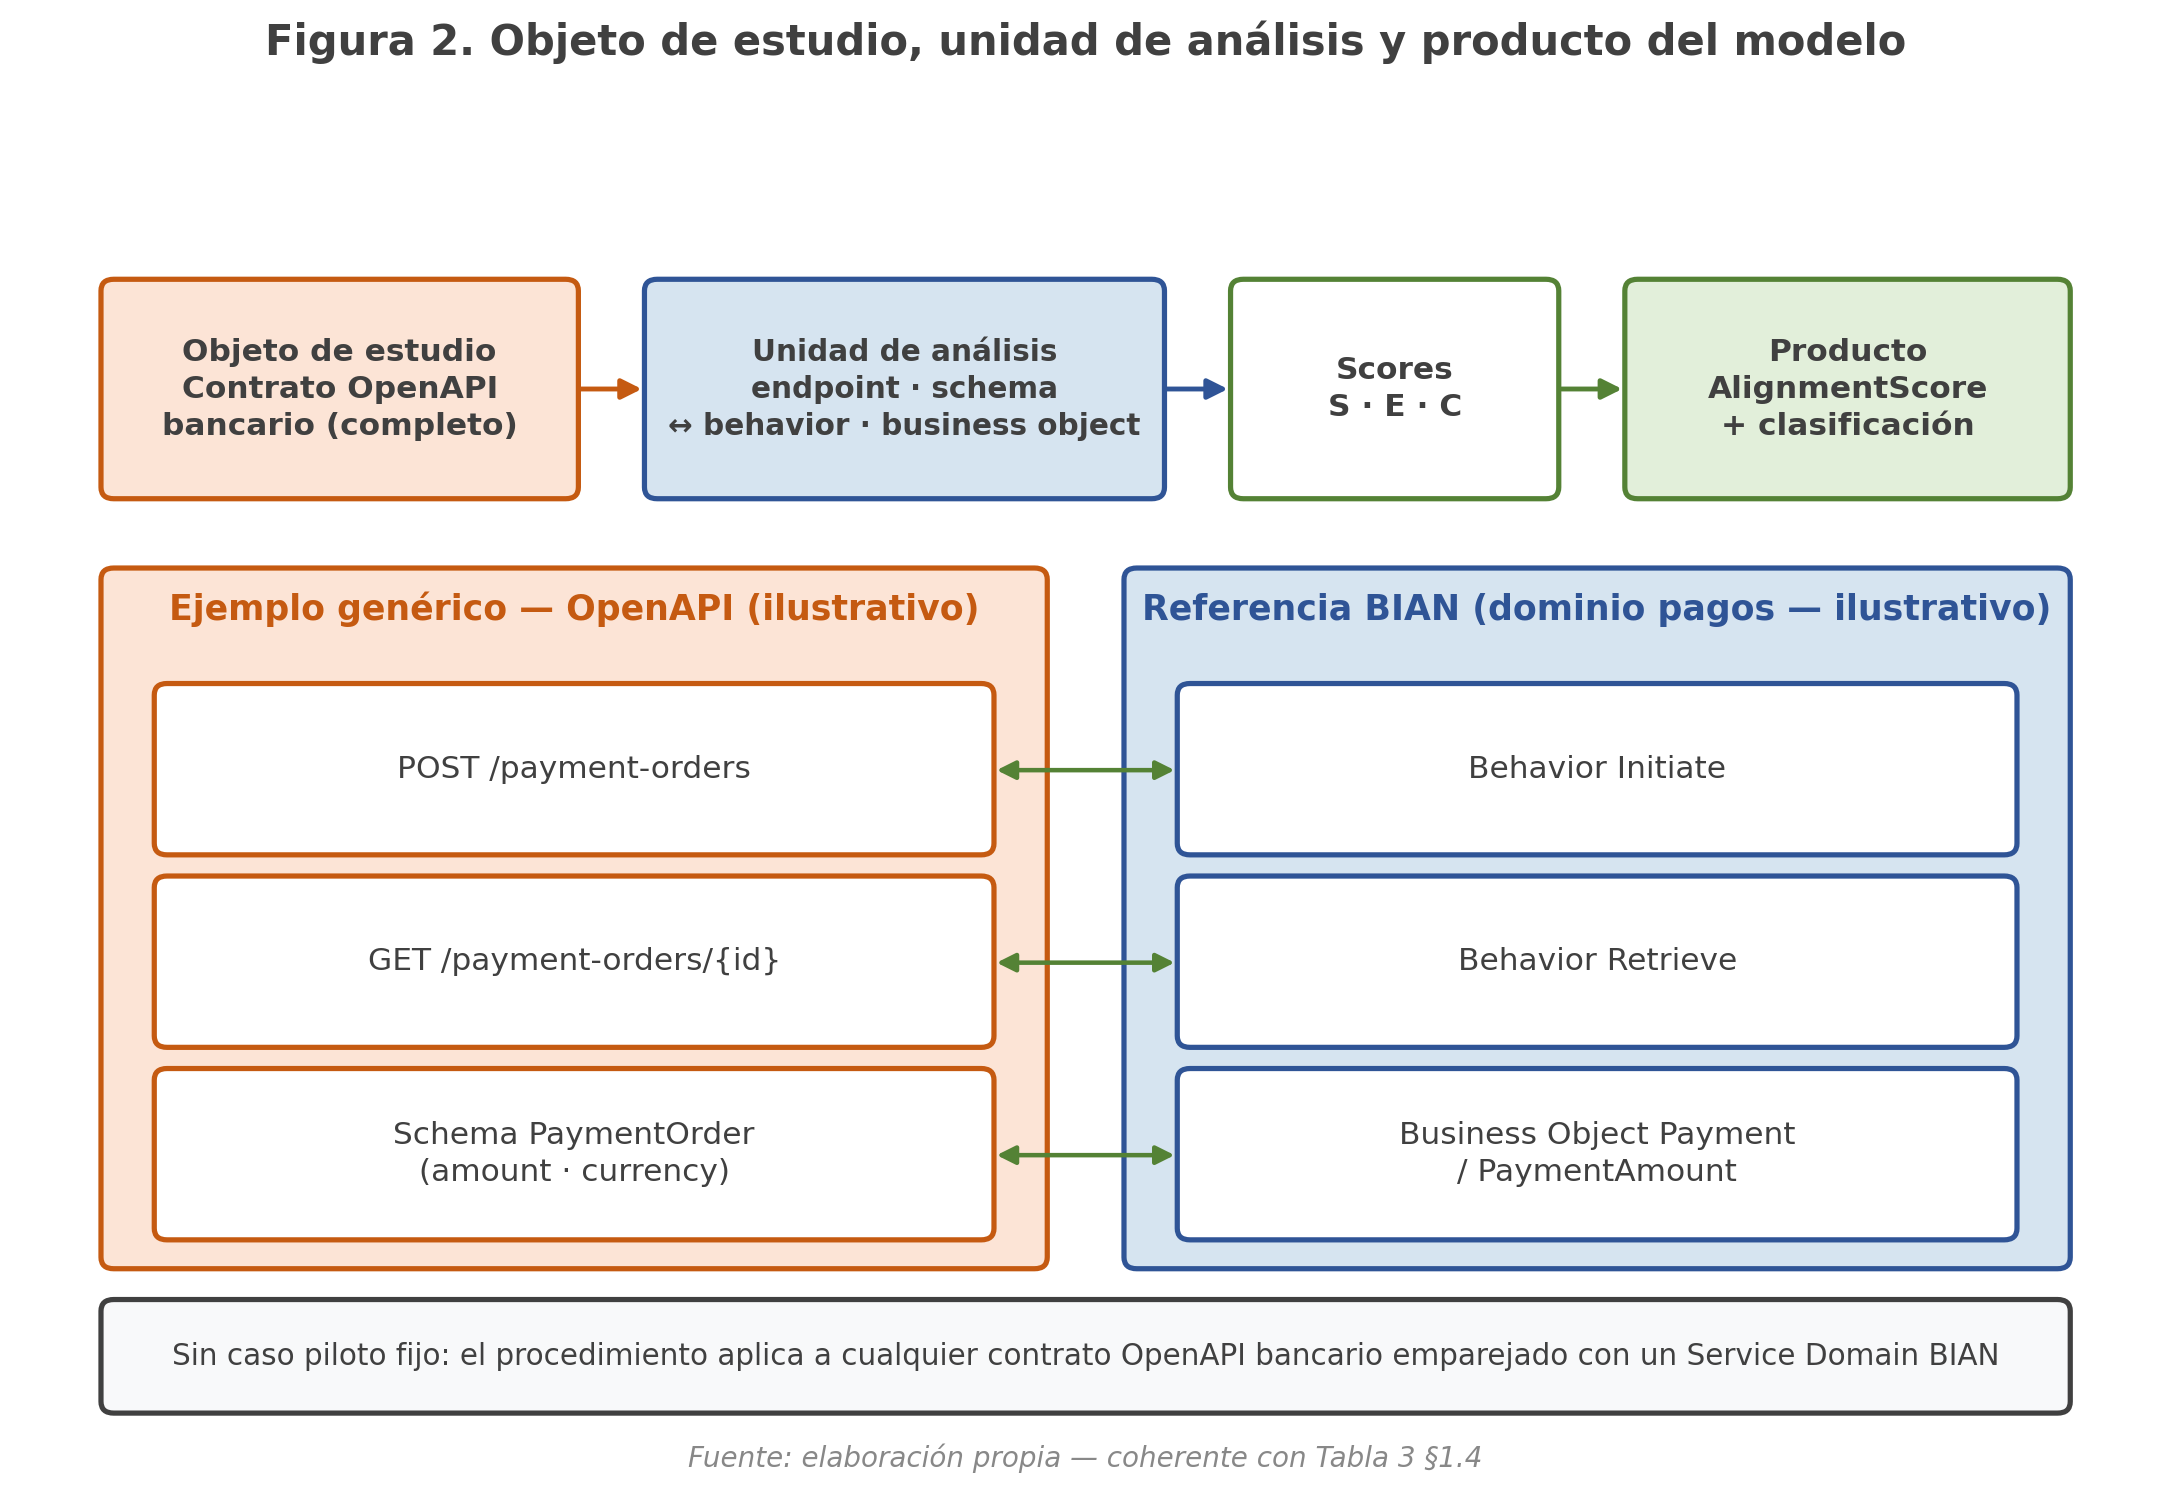
\includegraphics[width=0.88\textwidth]{Figura_02_Objeto_Unidad_Analisis}
  \caption{Objeto, referencia BIAN, unidad de análisis y producto del modelo}
  \label{fig:objeto}
\end{figure}

\begin{table}[H]
  \centering
  \caption{Objeto, unidad de análisis y producto}
  \label{tab:objeto}
  \begin{tabular}{@{}p{0.28\textwidth}p{0.62\textwidth}@{}}
    \toprule
    Concepto & En este estudio \\
    \midrule
    Objeto de estudio & El contrato OpenAPI bancario (el archivo) \\
    Unidad de análisis & Operación o esquema del contrato frente a un behavior o business object del Service Domain \\
    Producto & S, E, C y AlignmentScore por instancia contrato $\times$ dominio \\
    \bottomrule
  \end{tabular}
\end{table}

Cada instancia se nombra con la fuente, el dominio y la versión. I1 es \texttt{accounts} 2.4.2 contra Savings Account. El corpus público del capítulo III amplía las fuentes. No cambia el objeto.

\begin{table}[H]
  \centering
  \caption{Tipología de desalineaciones}
  \label{tab:tipologias}
  \small
  \begin{tabular}{@{}p{0.18\textwidth}p{0.38\textwidth}p{0.34\textwidth}@{}}
    \toprule
    Tipo & Qué es & Ejemplo \\
    \midrule
    Estructural & La organización de endpoints no sigue la del dominio & \texttt{POST /transfer} sin el behavior \texttt{Initiate} \\
    Semántica & La estructura se parece y el negocio no & \texttt{amount} sin vínculo con \texttt{PaymentAmount} \\
    De modelado & Falta una entidad o un atributo obligatorio & Un esquema que omite campos del business object \\
    REST / contrato & El verbo o la ruta no se leen como operación de negocio & Un verbo metido en la URL \\
    \bottomrule
  \end{tabular}
\end{table}

\section{Ámbito y delimitación}

El ámbito es el archivo público, no el banco. La tabla fija sector, artefactos, técnica, geografía y tiempo. Quedan fuera el despliegue, las pruebas de penetración y medir latencia en ejecución.

\begin{table}[H]
  \centering
  \caption{Ámbito del estudio}
  \label{tab:ambito}
  \begin{tabular}{@{}p{0.24\textwidth}p{0.66\textwidth}@{}}
    \toprule
    Dimensión & Delimitación \\
    \midrule
    Sector & Banca y servicios financieros con APIs \\
    Artefactos & Contratos OpenAPI o Swagger públicos, y Service Domains BIAN v14 \\
    Técnica & Análisis estructural y similitud semántica \\
    Geografía & No restringida. Los casos son documentación pública \\
    Tiempo & Especificaciones vigentes en 2024--2026. La lista de corpus se cerró el 21 de noviembre de 2026 \\
    \bottomrule
  \end{tabular}
\end{table}

\section{Alcances y limitaciones}
\label{sec:alcances}

El modelo ya está en un prototipo, y el piloto de siete instancias ya tiene número. La tabla separa eso de lo que sigue fuera: el YAML de un banco emisor, la corrida de todo el corpus contra los 258 dominios, y el despliegue. Los demás estándares públicos entran al corpus y, en este borrador, no tienen score.

\begin{table}[H]
  \centering
  \caption{Alcances y limitaciones}
  \label{tab:alcances}
  \footnotesize
  \begin{tabular}{@{}p{0.46\textwidth}p{0.46\textwidth}@{}}
    \toprule
    Alcance & Limitación \\
    \midrule
    Medir alineación estructural y semántica entre un contrato OpenAPI y un Service Domain & No desplegar APIs \\
    Dejar métricas que otra persona pueda repetir & No sustituir una certificación ni una auditoría legal \\
    El modelo S, E, C y el AlignmentScore & No puntuar los 258 dominios contra todo el corpus \\
    El corpus de contratos públicos del capítulo III & FDX y los PDF sin YAML no entran al parser \\
    El prototipo y el piloto de siete instancias, ya corrido & El resto del corpus todavía no tiene score \\
    Niveles Alta, Media, Baja y Nula & Los cortes son convención. No hay F1 \\
    \bottomrule
  \end{tabular}
\end{table}

\section{Justificación}

Si un release mueve el YAML y el Service Domain se queda en el modelo, el desfase se ve en el archivo: un path nuevo, un \texttt{operationId} que ya no nombra el behavior, un \texttt{\$ref} que apunta a otro esquema. Farzi \cite{Farzi2021} y Bhatia \cite{Bhatia2022} describen esa deriva entre producto, integración y gobernanza cuando el contrato y BIAN no se rastrean. Conviene verla en el archivo, no cuando el servicio ya está en producción.

Revisar a mano no escala cuando hay decenas de APIs y de socios. El AlignmentScore ordena esa cola con un número \cite{Shabbir2025}. OpenAPI, como artefacto, ya está maduro \cite{Casas2021}. Lo que no teníamos escrito es el cruce con un Service Domain. El procedimiento de esta tesis es esa pieza.

La pregunta cabe en el archivo. Este contrato, en esta versión, ¿refleja este Service Domain? S y E salen de ahí. No son una prueba en ejecución, ni un sello.

\section{Clasificación IEEE / ACM}

El tema cae en representación de conocimiento y en redes semánticas. No es testing de APIs ni un clasificador entrenado con nuestros pares.

\begin{table}[H]
  \centering
  \caption{Clasificación IEEE / ACM}
  \label{tab:clasificacion}
  \begin{tabular}{@{}p{0.16\textwidth}p{0.28\textwidth}p{0.46\textwidth}@{}}
    \toprule
    Taxonomía & Categoría & Por qué \\
    \midrule
    IEEE & Knowledge Representation &
    El contrato y el Service Domain son dos representaciones del mismo negocio. Medimos si se corresponden \\
    ACM & Semantic networks &
    El emparejamiento y la similitud entre conceptos de negocio y piezas de la API caen en redes de significado y en alineación de esquemas \\
    \bottomrule
  \end{tabular}
\end{table}

\section{Hipótesis de trabajo}

No las contrastamos en este borrador. Cada una nombra el producto de un objetivo y el ratio que se mediría cuando haya etiquetas.

\begin{enumerate}
  \item H1, ligada a OE1. Normalizar el contrato y el dominio en la misma tabla permite calcular S, E y C. El ratio es la completitud de la extracción.
  \item H2, ligada a OE2. El schema matching de Shvaiko y Euzenat \cite{Shvaiko2005} produce un StructuralScore de la correspondencia REST--dominio.
  \item H3, ligada a OE3. La similitud semántica \cite{ElBayadh2015,Chandrasekaran2022} produce un SemanticScore que separa un concepto alineado de uno que no lo está.
  \item H4, ligada a OE4. La media de S, E y C produce un AlignmentScore que se puede clasificar por nivel.
\end{enumerate}

\section{Factores y ratios}

Los factores son decisiones de diseño. Los ratios son los números. En esta corrida los factores ya están elegidos: tabla y no grafo, greedy con los pesos 0,40 / 0,25 / 0,20 / 0,15, S léxico y MiniLM, pesos iguales en el score oficial.

\begin{table}[H]
  \centering
  \caption{Factores y ratios}
  \label{tab:variables}
  \footnotesize
  \begin{tabular}{@{}p{0.12\textwidth}p{0.28\textwidth}p{0.24\textwidth}p{0.26\textwidth}@{}}
    \toprule
    Pieza & Factor & Ratio & Control \\
    \midrule
    OG & Pesos del AlignmentScore & Score y nivel & $\alpha+\beta+\gamma=1$. Cortes fijos \\
    OE1 & Representación intermedia & Extraídos / esperados & Versión fija del YAML y del dominio \\
    OE2 & Regla de matching & E en $[0,1]$ & Mismos pares normalizados \\
    OE3 & Encoder & S en $[0,1]$ & Mismos pares. Sin fine-tuning \\
    OE4 & Pesos & C, y el score global & Los tres pesos suman 1 \\
    \bottomrule
  \end{tabular}
\end{table}

\begin{figure}[H]
  \centering
  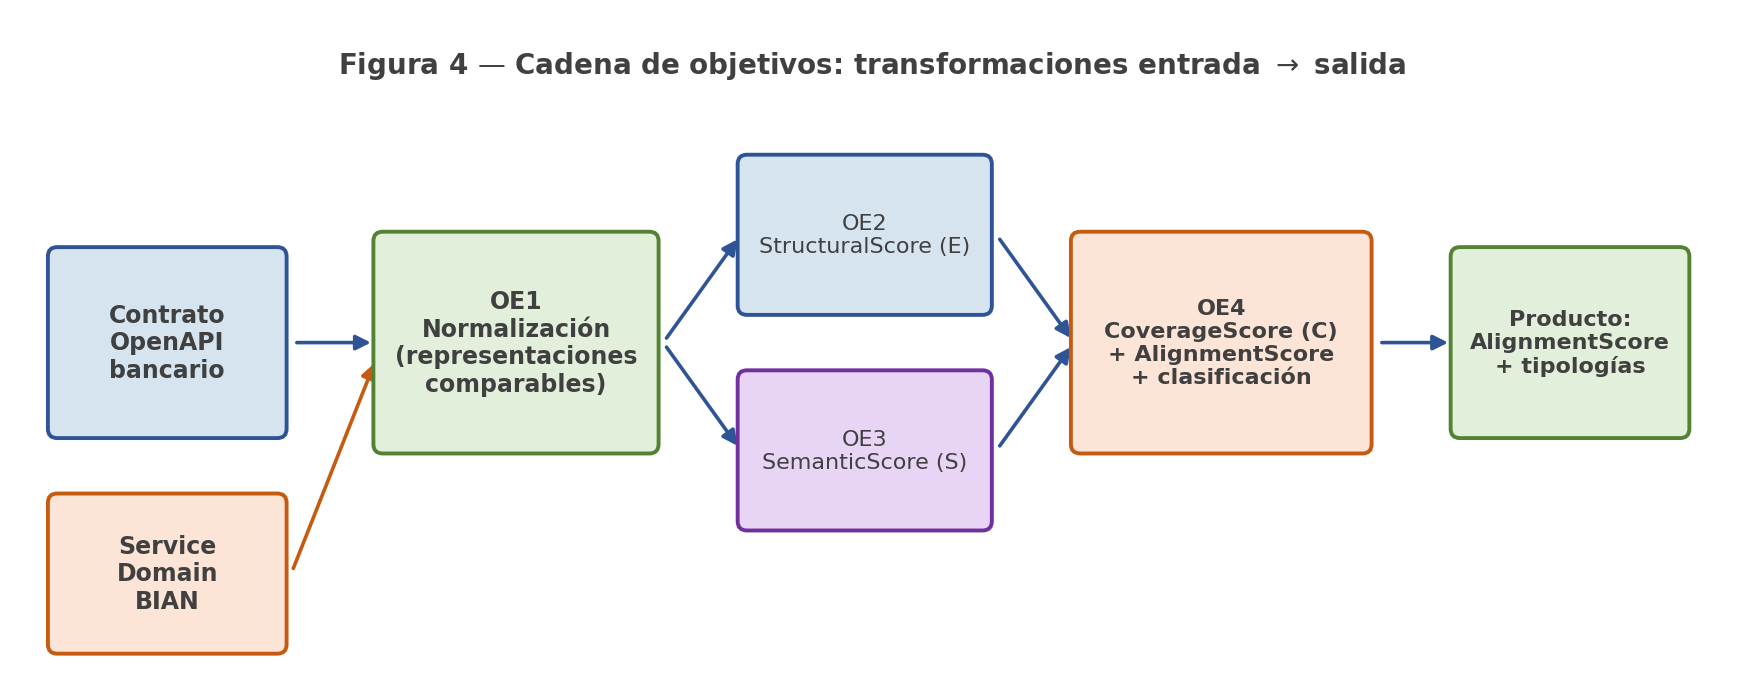
\includegraphics[width=0.98\textwidth]{Figura_04_Cadena_Objetivos}
  \caption{Cadena: normalizar, calcular S, E y C, integrar el AlignmentScore}
  \label{fig:cadena}
\end{figure}
